\documentclass[tikz,border=6pt]{standalone}
\usetikzlibrary{arrows.meta}
\definecolor{red}{HTML}{A50F2D}\definecolor{ink}{HTML}{141414}\definecolor{gry}{HTML}{5F5F5F}\definecolor{blu}{HTML}{2B6CB0}\definecolor{teal}{HTML}{1B9E8F}
\begin{document}
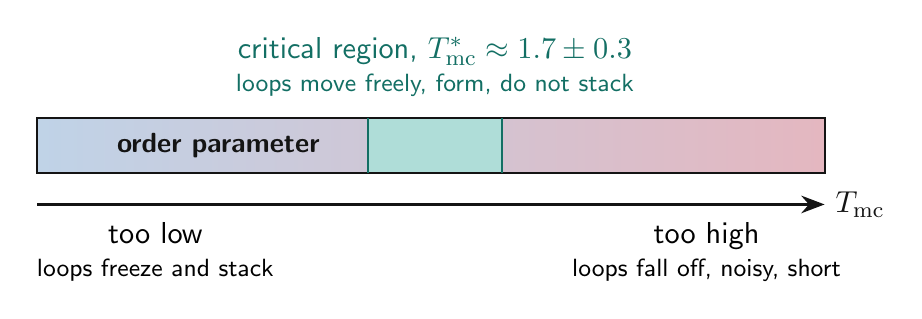
\begin{tikzpicture}[font=\sffamily\fontsize{11}{13}\selectfont,>=Stealth]
% bar: frozen (left) - critical region (middle) - noisy (right)
\shade[left color=blu!30,right color=red!30] (0,0) rectangle (10,0.7);
\fill[teal!35] (4.2,0) rectangle (5.9,0.7);
\draw[ink,thick] (0,0) rectangle (10,0.7);
\draw[teal!70!black,thick] (4.2,0)--(4.2,0.7); \draw[teal!70!black,thick] (5.9,0)--(5.9,0.7);
\draw[->,ink,very thick] (0,-0.4)--(10,-0.4) node[right]{$T_{\mathrm{mc}}$};
\node[anchor=north,align=center] at (1.5,-0.5) {too low\\[-1pt]\small loops freeze and stack};
\node[anchor=north,align=center] at (8.5,-0.5) {too high\\[-1pt]\small loops fall off, noisy, short};
\node[teal!70!black,anchor=south,align=center] at (5.05,0.85) {critical region, $T^*_{\mathrm{mc}}\approx 1.7\pm 0.3$\\[-1pt]\small loops move freely, form, do not stack};
\node[ink,font=\sffamily\bfseries] at (2.3,0.35) {order parameter};
\end{tikzpicture}
\end{document}
